\chapter{Referencial teórico}

O referencial teórico revela o momento de levantar o embasamento teórico sobre o tema de pesquisa. No contexto desse TCC, faz-se necessário, dentros outros aspectos pesquisar sobre os entendimentos existentes do problema de pesquisa e analisar quais mecanismos devem ser adotados para se propor uma solução \cite{belchior2012}.

O referencial teórico deste TCC irá levantar o embasamento teórico sobre Contexto Financeiro, Métodos Matemáticos, Paradigmas de Programação e Testes estáticos/dinâmicos para que seja possível propor uma solução para o problema de pesquisa.

\section{Contexto Financeiro}
Esta seção irá tratar os atributos aliados ao contexto financeiro como Alavancagem, Suporte e Resistência. Esses atributos são insumos para que se possa compreender melhor a dinâmica das estratégias para negociação no Mercado de Moedas.

\subsection{Mercado de Moedas}
Mercado de Moedas ou FOREX (abreviatura de Foreign Exchange) é um mercado interbancário onde as várias moedas do mundo são negociadas. O FOREX foi criado em 1971, quando a negociação internacional transitou de taxas de câmbio fixas para flutuantes. Com o resultado do seu alto volume de negociações, o Mercado de Moedas tornou-se o principal mercado financeiro do mundo \cite{market2011}.

A operação no Mercado de Moedas envolve a compra de uma moeda e a simultânea venda de outra. As moedas são negociadas em pares, por exemplo: euro e dólar (EUR-USD). O investidor não compra ou vende euro e dólares fisicamente, mas existe uma relação monetária de troca entre eles. O FOREX é um mercado em que são negociados, portanto, derivativos de moedas. O investidor é remunerado pelas diferenças entre a valorização (se tiver comprado) ou desvalorização (se tiver vendido) destas moedas \cite[pág.~3]{cvm2009}.

O Mercado de Moedas é descentralizado, pois as operações são realizadas por vários participantes do mercado em vários locais. É raro uma moeda manter uma cotação constante em relação a outra moeda. O câmbio entre duas moedas muda constantemente \cite[pág.~5]{fxcm2011}.

O Mercado de Moedas é constituído por transações entre as corretoras que operam no mesmo e são negociados, diariamente, contratos representando volume total entre 1 e 3 trilhões de dólares. As transações são realizadas diretamente entre as partes (investidor e corretora) por telefone e sistemas eletrônicos, desde que tenham conexão à internet. As operações ocorrem 24 horas por dia, durante 5 dias da semana (abrindo às 18h no domingo e fechando às 18h na sexta; horário de Brasília), negociando os principais pares de moedas, ao redor do mundo \cite[pág.~4]{cvm2009}.

\subsection{Alavancagem}
Alavancagem no contexto de mercado,deriva do significado de alavanca na Física, relacionado com a obtenção de um resultado final maior do que ao esforço empregado \cite[pág.~3]{dantas2006}.

\begin{citacao}
O conceito de alavancagem é similar ao conceito de alavanca comumente empregado em física. Por meio da aplicação de uma força pequena no braço maior da alavanca, é possível mover um peso muito maior no braço menor da alavanca \cite[pág.~232]{bruni2011}.
\end{citacao}

A Alavancagem possui a propriedade de gerar oportunidades financeiras para empresas que possuem indisponibilidade de recursos internos e/ou próprios \cite[p~13]{albuquerque2013}.

No mercado FOREX, o investidor pode negociar contratos de taxas de câmbio e usar a Alavancagem para aumentar suas taxas de lucro. Se o investidor, por exemplo, realizar uma operação de compra apostando 0.01 por ponto e o mercado subir 1000 pontos, ele ganha 10 dólares (0.001x1000). Usando a técnica de Alavancagem, o investidor pode realizar a mesma operação de compra colocando sua operação alavancada a 1.0, realizando o lucro de 1000 dólares (1.0x1000) \cite{easyforex2014}.

\subsection{Suporte}

Segundo \citeonline[pág.~22]{matsura2006},  Suporte é o nível de preço no qual a pressão compradora supera a vendedora e interrompe o movimento de baixa. Pode-se identificar o Suporte por uma linha reta horizontal conforme a figura \ref{retaSuporte}.

\begin{figure}[htp]
\centering
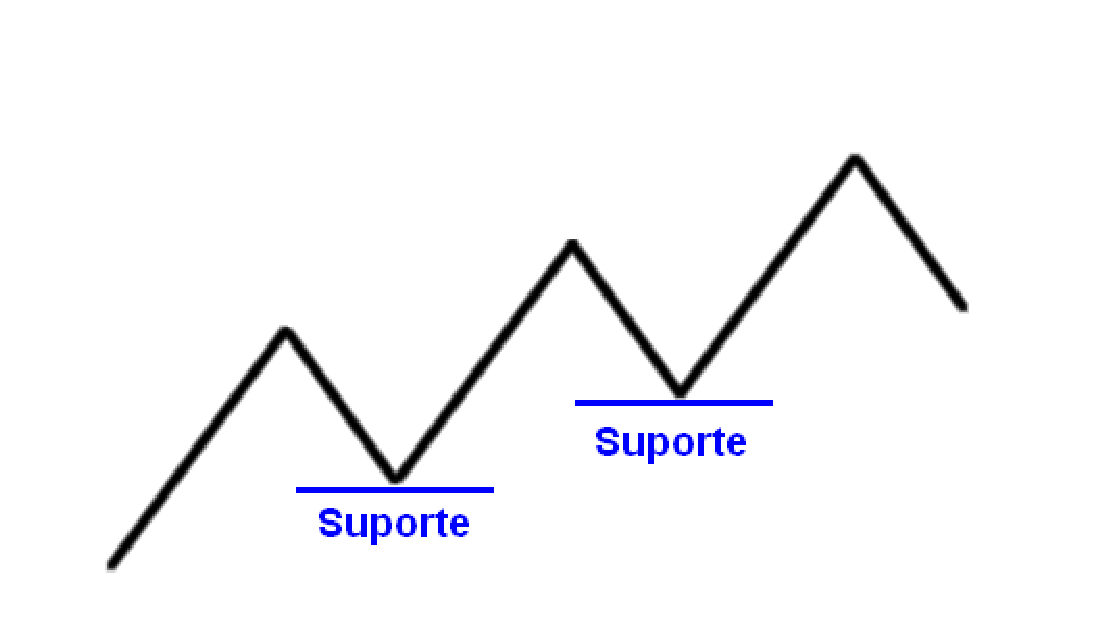
\includegraphics[width=0.9\textwidth]{figuras/retaSuporte}
\caption{Reta de Suporte.}{Fonte: \citeonline[pág.~22]{matsura2006}.}
\label{retaSuporte}
\end{figure}

Suporte é uma região gráfica que após uma queda, os preços param e revertem no sentido contrário. É uma área em que os investidores tendem a comprar \cite[p~97]{debastini2008}.

Os níveis de Suporte indicam as cotações em que os investidores acreditam que vão subir. À medida em que as cotações se deslocam para a zona de Suporte, os investidores estão mais confiantes para comprar \cite{collins2012}.

\subsection{Resistência}

Resistência é a região do gráfico em que após um movimento de alta, os preços param e revertem no sentido contrário. É um ponto em que os investidores tende a vender para ter o maior lucro possível \cite[pág.~98]{debastini2008}.

Segundo \citeonline[pág.~23]{matsura2006}, Resistência representa o nível de preço no qual a pressão vendedora supera a compradora e interrompe o movimento de alta. A Resistência é identificada por uma linha reta horizontal, conforme a figura \ref{retaResistencia}.

\begin{figure}[htp]
\centering
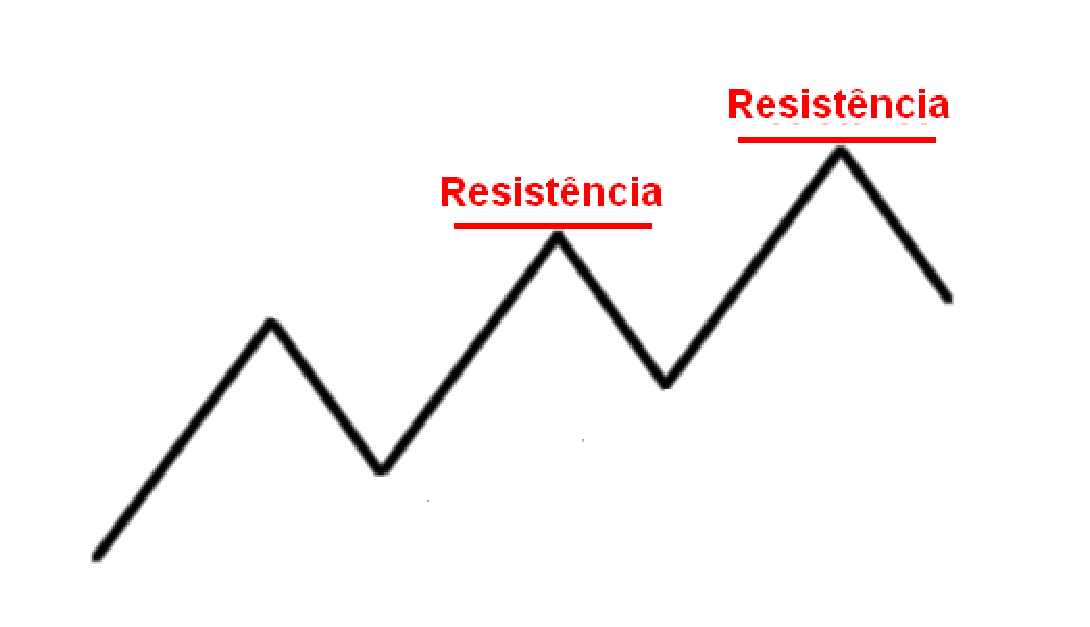
\includegraphics[width=0.7\textwidth]{figuras/retaResistencia}
\caption{Reta de Resistência.}{Fonte: \citeonline[pág.~23]{matsura2006}} 
\label{retaResistencia}
\end{figure}

A Resistência indica os níveis das cotações em que os investidores acreditam que as mesmas vão descer. À medida que as cotações se deslocam para a zona de Resistência, os investidores estão mais confiantes para vender \cite{collins2012}.

\section{Métodos Matemáticos}

Métodos Matemáticos é qualquer método que se utiliza da matemática para resolver um problema. É possível citar alguns exemplos desses métodos como equações polinomiais, identidades trigonométricas, geometria coordenada, frações parciais, expansões binomiais, entre outros \cite{riley2011}.

Métodos Matemáticos são aplicados a área de finanças. Cálculo e álgebra linear são fundamentais para o estudo de matemática financeira e ajuda a compreender a dinâmica de mercado \cite{konis2014}.

Este capítulo irá abordar sobre os Métodos Matemáticos de Mínimos Quadrados, Fibonacci e Correlação Linear de Pearson.

\subsection{Método de Mínimos Quadrados}

O método de Mínimos Quadrados determina o valor mais provável de quantidades não conhecidas em que a soma dos quadrados das diferenças entre valores observados e computados é mínimo \cite[pág.~72]{inacio2010}.

Usa-se o método de Mínimos Quadrados para determinar a melhor linha de ajuste que passa mais perto de todos os dados coletados, no intuito de obter a melhor linha de ajuste, de forma que minimize as distâncias entre cada ponto de consumo \cite[pág.~46]{dias1985}.

A aplicação do método de Mínimos Quadrados visa deduzir a melhor estimativa de mensurações de n medições idênticas (em condições de “repetitividade”) e não idênticas (em condições de “reprodutividade”). Dessa forma o peso estatístico de um resultado é definido \cite[pág.~149]{vuolo1996}.

O desvio vertical do ponto:
\begin{equation}
(x_{i}, y_{i})
\end{equation}
da reta:
\begin{equation}
Y = B0 = B1*X_{i}
\end{equation}
é a altura do ponto menos altura da reta. A soma dos desvios quadrados verticais dos pontos:
\begin{equation}
(x_{1}, y_{1})...(x_{i}, y_{i})
\end{equation}
à reta é portanto:
\begin{equation}
f(B0,B1) = \sum{y_{i} - (B0 + B1 * X_{i})}^2
\end{equation}
\begin{equation}
0 <= i > \infty
\end{equation}

As estimativas pontuais de C0 e C1, representadas por K0 e K1 e denominadas estimativa de Mínimos Quadrados, são aquelas que minimizam f(B0, B1). Em suma,  para qualquer B0 e B1, K0 e K1 são tais que:
\begin{equation}
f(K0,K1) <= f(B0,B1)
\end{equation}

A reta de Regressão Estimativa ou de Mínimos Quadrados é, por conseguinte, a reta cuja equação é :
\begin{equation}
Y = K0 + K1X 
\end{equation}
Como mostrado na figura \ref{equacaoMinimos}\cite[pág.~441]{devore2006}.

\graphicspath{{figuras/}}
\begin{figure}[htp]
\centering
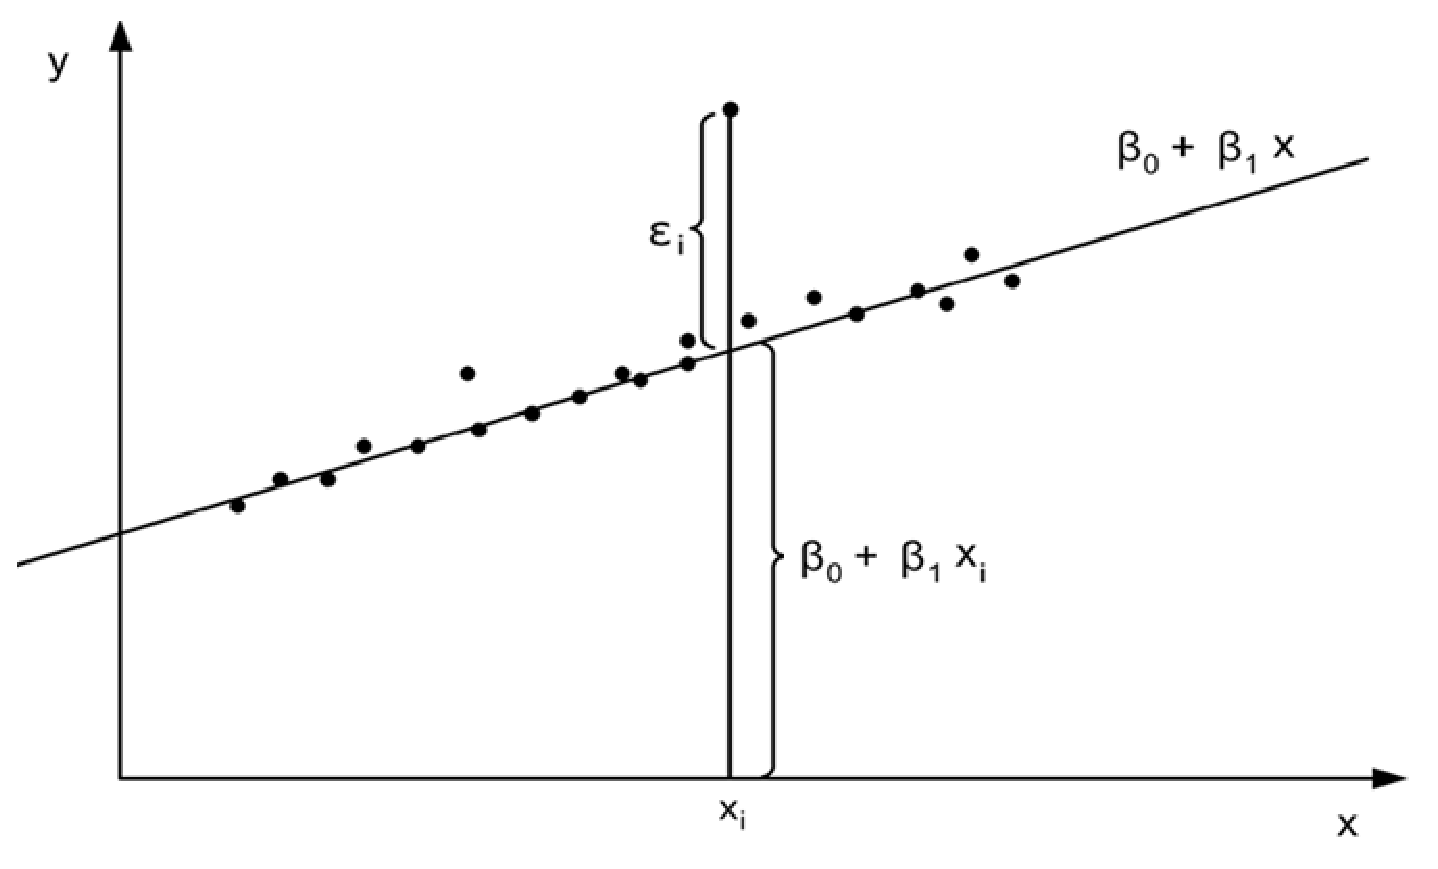
\includegraphics[width=0.9\textwidth]{equacaoMinimosQuadrados}
\caption{Equação da reta Mínimos Quadrados.}{Fonte: \citeonline[pág.~443]{devore2006}.} 
\label{equacaoMinimos}
\end{figure}

\subsection{Método de Correlação Linear}

Em estudos que envolvem duas ou mais variáveis, é comum o interesse em conhecer o relacionamento entre elas, além das estatísticas descritivas normalmente calculadas. A medida que mostra o grau de relacionamento entre as variáveis é chamada de Coeficiente de Correlação ou Correlação Linear ou Correlação Linear de Pearson. A Correlação Linear também é conhecida como medida de associação, interdependência, intercorrelação ou relação entre as variáveis \cite[pág.~62]{lira2004}.

O Coeficiente de Correlação Linear de Pearson (r) é uma estatística utilizada para medir força, intensidade ou grau de relação linear entre duas variáveis aleatórias \cite[pág.~664]{ferreira2009}.

Segundo \cite[pág.~134]{lopes2005}, a Correlação Linear indica a relação entre duas variáveis. De modo a interpretar o coeficiente de correlação (r), podem ser utilizados os seguintes critérios para classificar os resultados obtidos:

\begin{itemize}
\item De 0 a 0,50: fraca correlação; 
\item De 0,51 a 0,84: moderada correlação;
\item A partir de 0,85: forte correlação.
\end{itemize}

\graphicspath{{figuras/}}
\begin{figure}[htp]
\centering
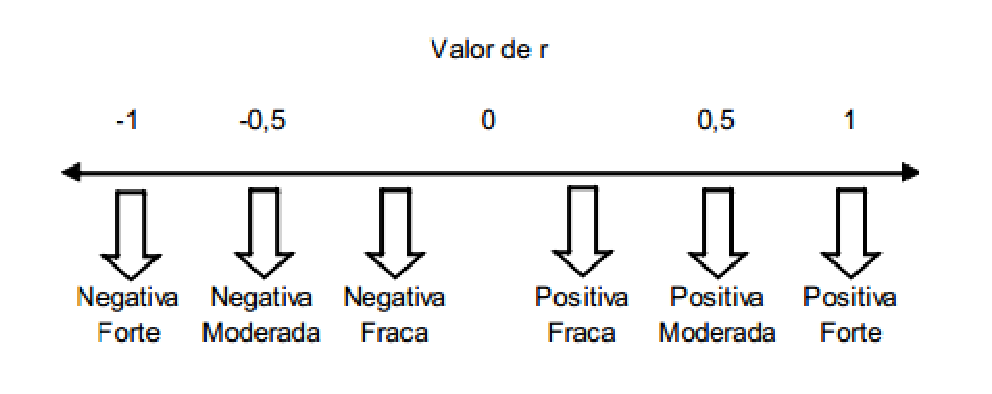
\includegraphics[width=0.9\textwidth]{classificacaoCorrelacaoLinear}
\caption{Classificação da Correlação Linear.}{Fonte: \citeonline[pág.~134]{lopes2005}.} 
\label{classificacaoCorrelacaoLinear}
\end{figure}

Segundo \citeonline[pág.~47]{regra2010} a Correlação Linear revela o grau de associação entre duas variáveis aleatórias. A dependência de duas variáveis X e Y é dada pelo Coeficiente de Correlação Amostral, conhecido também por coeficiente r-de-Pearson. Designa-se, normalmente, por r e é determinado de acordo com a figura \ref{determinacaoCorrelacao}.

\begin{figure}[htp]
\centering
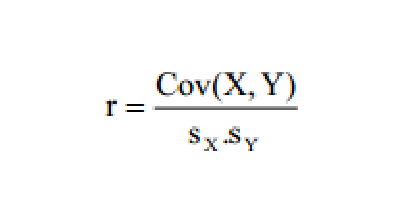
\includegraphics[width=0.5\textwidth]{figuras/determinacaoCorrelacao1}
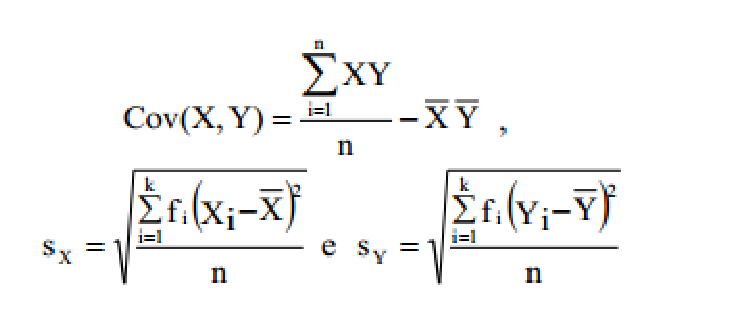
\includegraphics[width=0.9\textwidth]{figuras/determinacaoCorrelacao2}
\caption{Determinação da Correlação Linear.}{Fonte: \citeonline{regra2010}.}
\label{determinacaoCorrelacao}
\end{figure}

Segundo \citeonline[pág.~8]{viali2009} as propriedades mais importantes do Coeficiente de Correlação são:

\begin{enumerate}
\item O intervalo de variação vai de -1 a +1.
\item O coeficiente é uma medida adimensional, isto é, independente das unidades de medida das variáveis X e Y.
\item  Quanto mais próximo de +1 for “r”, maior o grau de relacionamento linear positivo entre X e Y, ou seja, se X varia em uma direção, Y variará no mesmo sentido.
\item Quanto mais próximo de -1 for “r”, maior o grau de relacionamento linear negativo entre X e Y, isto é, se X varia em um sentido, Y variará na direção inversa.
\item Quanto mais próximo de zero estiver “r”, menor será o relacionamento linear entre X e Y. Um valor igual a zero indicará ausência apenas de relacionamento linear.
\end{enumerate}

A análise da Correlação Linear fornece um número, indicando como duas variáveis variam conjuntamente e mede a intensidade e a direção da relação linear ou não-linear entre duas variáveis. Essa análise também é um indicador que atende à necessidade de estabelecer a existência ou não de uma relação entre essas variáveis sem que, para isso, seja preciso o ajuste de uma função matemática. Em suma, o grau de variação conjunta entre X e Y é igual ao de Y e X \cite[pág.~65]{lira2004}.

\subsection{Método de Fibonacci}

A sucessão ou sequência de Fibonacci é uma sequência de números naturais, na qual os primeiros dois termos são 0 e 1, e cada termo subsequente corresponde à soma dos dois precedentes. A sequência tem o nome do matemático pisano do século XIII Leonardo de Pisa,  conhecido como Leonardo Fibonacci, e os termos são chamados números de Fibonacci. Os números de Fibonacci compõem a seguinte sequência de números inteiros: 0, 1, 1, 2, 3, 5, 8, 13, 21, 34, 55, 89, 144, …, \cite[pág.~6]{gagliardi2013}.

Devido a sequência de Fibonacci ser recursiva, é possível determinar uma fórmula capaz de encontrar o valor de qualquer número de Fibonacci, Fn, se seu lugar na sequência, n, for conhecido. Esta propriedade garante que para obter todas as soluções da equação recursiva de Fibonacci: Fn+1 = Fn-1 + Fn, para qualquer n > 1 \cite[pág.~12]{sousa2012}.

Segundo \citeonline[pág.~32]{rocha2008}, a fórmula de Fibonacci, sem uso da recorrência, é dada de acordo com a figura \ref{formulaFibonacci}. Essa fórmula também é conhecida como fórmula de Binet.

\begin{figure}[htp]
\centering
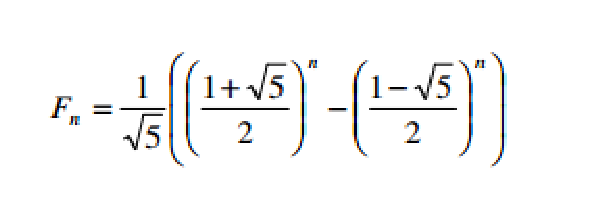
\includegraphics[width=0.9\textwidth]{figuras/formulaFibonacci}
\caption{Fórmula de Fibonacci sem uso de recorrência.}{Fonte: \citeonline[pág.~32]{rocha2008}.} 
\label{formulaFibonacci}
\end{figure}

\section{Paradigmas de Programação}

A palavra paradigma significa aquilo que pode ser utilizado como padrão, de forma que é um modelo a ser seguido \cite{ferreira1986}. Segundo \citeonline{normak2013} Kurt Normark (2013), professor da Universidade de Aalborg na Dinamarca, paradigma de programação é um padrão que serve como uma escola de pensamentos para a programação de computadores.



Uma linguagem de programação multiparadigma é uma linguagem de programação que suporta mais de um paradigma de programação. O objetivo de tais linguagens é permitir que programadores usem a melhor ferramenta para o trabalho, admitindo que nenhum paradigma  resolve todos os problemas da maneira mais fácil ou mais eficiente \cite[pág.~21]{paquet2010}. Seguem noções preliminares sobre cada paradigma, os quais serão investigados ao longo desse TCC.

\subsection{Paradigma Procedural}

Programação procedural é um paradigma de programação, derivado da programação estruturada, com base no conceito da chamada de procedimento. Procedimentos, também conhecidos como rotinas, sub-rotinas, métodos ou funções, contêm uma série de passos computacionais a serem realizados. Qualquer procedimento pode ser chamado a qualquer momento durante a execução de um programa, inclusive por outros procedimentos ou a si mesmo \cite[pág.~22]{paquet2010}.

A linguagem de programação procedural fornece ao programador  um meio de definir com precisão cada passo na execução de uma tarefa e é muitas vezes uma escolha melhor em situações que envolvem complexidade moderada ou que requerem significativa facilidade de manutenção \cite[pág.~22]{paquet2010}.

As linguagens procedurais foram desenvolvidas em torno da arquitetura de computadores prevalentes na época, chamada de  arquitetura von Neumann, criada pelo matemático húngaro John von Neumann \cite[pág.~18]{sebesta2012}.

Em um computador de von Neumann, ambos os dados e programas são armazenados na mesma memória. A unidade central de processamento (CPU), que executa as instruções, é separada da memória. Portanto, as instruções e os dados devem ser transmitidos da memória para a CPU. Os resultados das operações na CPU devem ser devolvidos à memória, conforme ilustra a figura \ref{arquiteturaVon}.

\begin{figure}[htp]
\centering
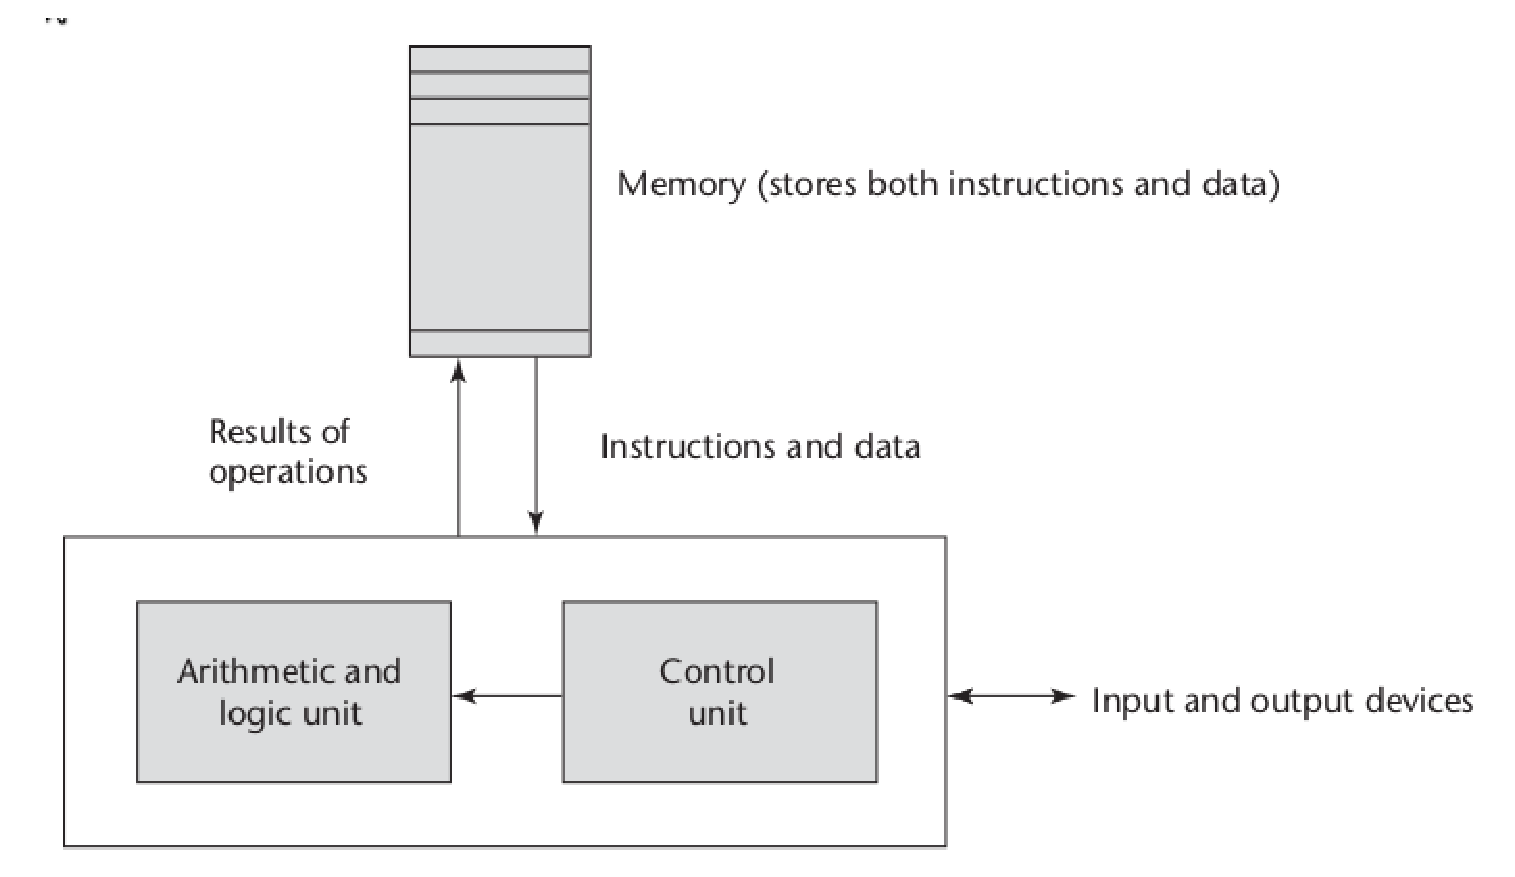
\includegraphics[width=0.9\textwidth]{figuras/arquiteturaVon}
\caption{Arquitetura de von Neumann.}{Fonte: \citeonline[pág.~19]{sebesta2012}.}
\label{arquiteturaVon}
\end{figure}

Devido ao uso da arquitetura de von Neumann, os recursos centrais das linguagens imperativas são as variáveis, as quais modelam as células de memória, as instruções de atribuição, baseadas na operação de canalização (piping) e na forma interativa de repetição, o método mais eficiente dessa arquitetura. A iteração é rápida nos computadores de von Neumann uma vez que as instruções são armazenadas em células adjacentes da memória. Esta eficiência desencoraja o uso de recursão para repetição, embora a recursão seja frequentemente mais natural \cite[pág.~18]{sebesta2012}.

Linguagens imperativas contêm variáveis e valores inteiros, operações aritiméticas básicas, comandos de atribuição, sequenciamentos de comandos baseados em memórias, condições e comandos de ramificação. Essas linguagens suportam determinadas características comuns, que surgiram com a evolução do paradigma, tais como: estruturas de controle, entrada/saídas, manipulação de exceções e erros, abstração procedural, expressões e atribuição, e suporte de biblioteca para estruturas de dados \cite[pág.~278-279]{tucker2009}.

Fortran (FORmula TRANslation) foi a primeira linguagem de alto nível a ganhar ampla aceitação, sendo esta uma linguagem imperativa. Projetada para aplicações científicas, essa linguagem conta com notação algébrica, tipos, subprogramas e entrada/saída formatada. Foi implementada em 1956 por John Backus na IBM especificamente para a máquina IBM 704. A execução eficiente foi uma grande preocupação, consequentemente, sua estrutura e comandos têm muito em comum com linguagens de montagem \cite[pág.~458]{brookshear}.

Outra linguagem de programação é o C \citeonline{ritchie1996}, um dos criadores da linguagem, ela se tornou uma linguagem dominante na década de 90. Seu sucesso deve-se ao sucesso do Unix, um sistema operacional implementado em C.

\begin{citacao}
Apesar de alguns aspectos misteriosos para o iniciante e ocasionalmente até mesmo para o adepto, a linguagem C permanece uma simples e pequena linguagem, traduzível com simples e pequenos compiladores. Seus tipos e operações são bem fundamentados naquelas fornecidas por máquinas reais, e para pessoas que usam o OO computador para trabalhar, aprender a linguagem para gerar programas em tempo – e espaço – eficientes não é difícil. Ao mesmo tempo a linguagem é suficientemente abstrata dos detalhes da máquina de modo que a portabilidade de programa pode ser alcançada \cite{ritchie1996}.
\end{citacao}

\subsection{Paradigma Orientado a Objetos}

Um objeto é a abstração de uma "coisa" (alguém ou algo), e esta abstração é expressa com a ajuda de uma linguagem de programação. A coisa pode ser um objeto real, ou algum conceito mais complicado. Tomando um objeto comum, como um gato, por exemplo, você pode ver que ele tem certas características (cor, nome, peso) e pode executar algumas ações (miar, dormir, esconder, fugir). As características do objeto são chamados de propriedades em Orientação a Objetos (OO) e as ações são chamadas de métodos \cite[pág.~13]{stefanov2008}.

O conceito de objeto não surgiu do paradigma orientado a objetos. Pode-se dizer ainda que OO foi uma evolução das práticas já existentes da época. O termo objetos surgiu quase simultaneamente em 1970 em vários ramos da ciência da computação, algumas áreas que influenciaram o paradigma OO foram: sistemas de simulação, sistemas operacionais, abstração de dados e inteligência artificial, como ilustra a figura \ref{essenciaOO} \cite[pág.~1]{capretz2003}.

\begin{figure}[htp]
\centering
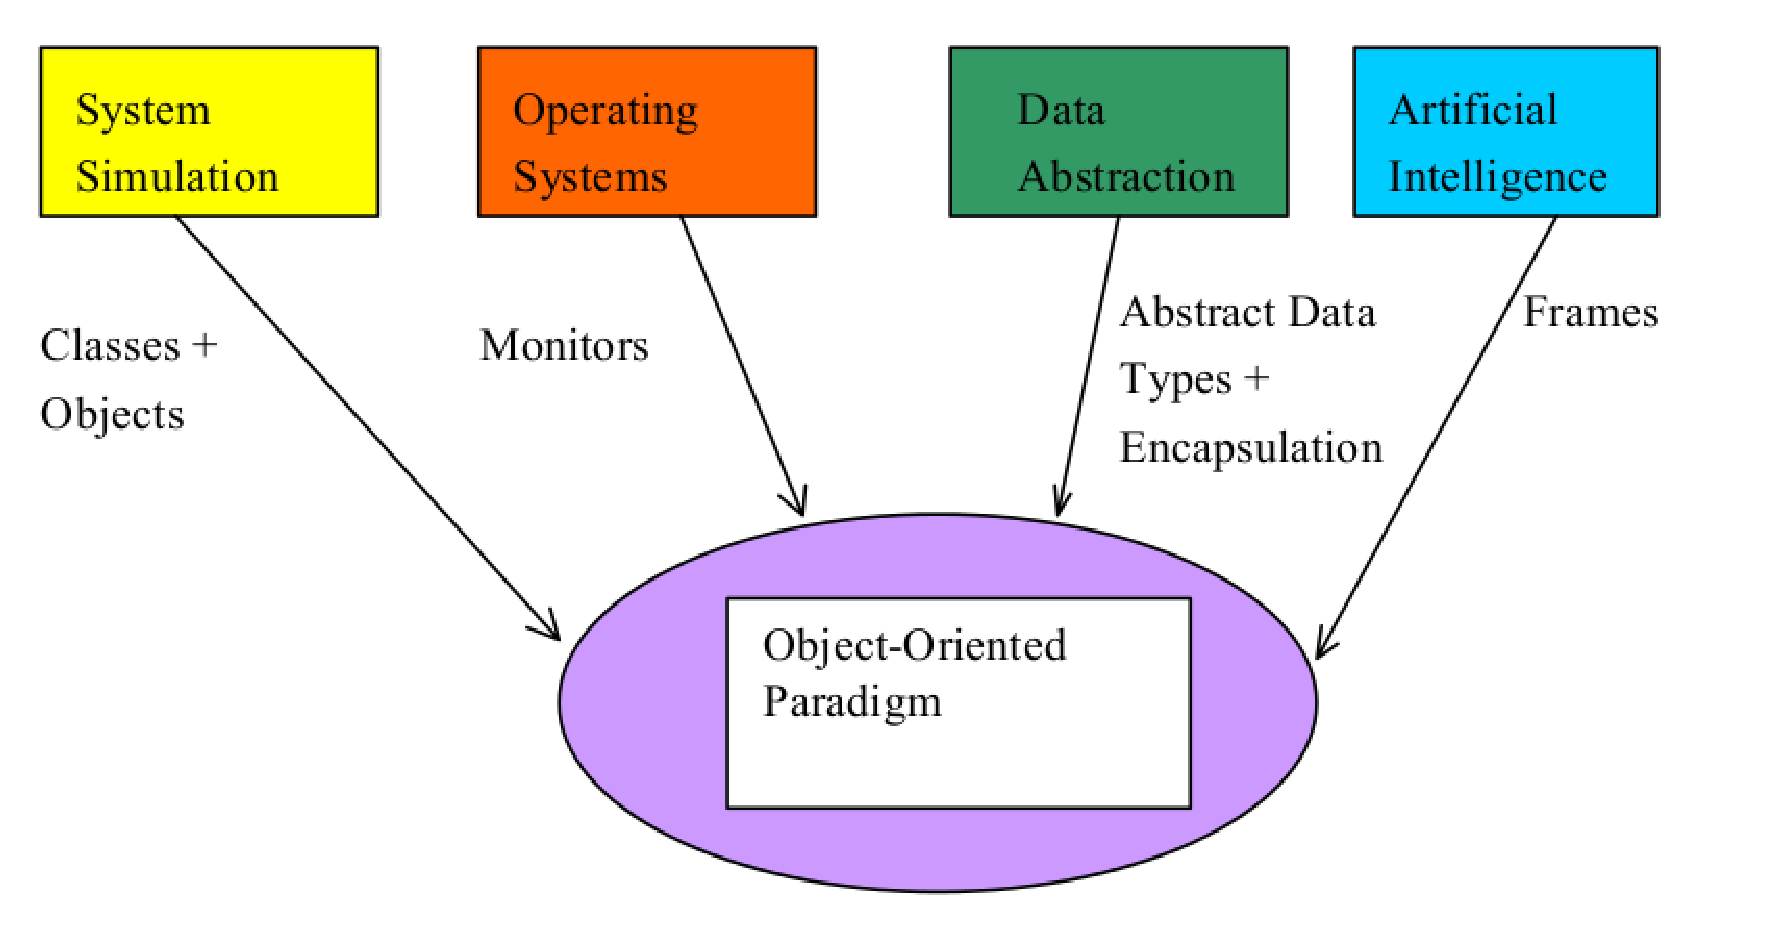
\includegraphics[width=0.9\textwidth]{figuras/essenciaOO}
\caption{A essência do Paradigma Orientado a Objetos.}{Fonte: \citeonline[pág.~1]{capretz2003}.} 
\label{essenciaOO}
\end{figure}

A programação orientada a objetos fornece um modelo no qual um programa é uma coleção de objetos que interagem entre si, passando mensagens que transformam seu estado. Neste sentido, a passagem de mensagens permite que os objetos dados se tornem ativos em vez de passivos \cite[pág.~310]{tucker2009}.

Classes servem como modelos a partir dos quais objetos podem ser criados. Elas tem precisamente as mesmas variáveise operações de instâncias dos objetos, mas sua interpretação é diferente: onde um objeto representa variáveis reais, variáveis de classe são, em potencial, instanciadas apenas quando um objeto é criado  \cite[pág.~10]{wegner1990}.

Uma das principais vantagens do uso de orientação a objetos é que o objeto não precisa revelar todos os seus atributos e comportamentos (métodos). Em um bom design OO um objeto só deve revelar as interfaces necessárias para interagir com outros objetos. Os detalhes não pertinentes para a utilização do objeto deve ser ocultado de todos os outros objetos. Por exemplo, um objeto que calcula o quadrado de um número deve fornecer uma interface para obter o resultado. No entanto, as propriedades internas e algoritmos utilizados para calcular o quadrado não têm de ser disponibilizados ao objeto solicitante. O encapsulamento  é definido pelo fato de que os objetos envolvem (quase que como uma cápsula) atributos e métodos, e a ocultação de dados é uma das partes mais importantes do encapsulamento \cite[pág.~19]{weisfeld2009}.

Uma nova classe (designada por subclasse derivada) pode ser derivada de outra classe (designada por superclasse) por um mecanismo chamado de herança. A classe derivada herda todas as características da classe base: a sua estrutura e comportamento (resposta a mensagens). Além disso, o mecanismo de herança é permitido mesmo sem acesso ao código-fonte da classe base. Herança dá a OO seu benefício chefe sobre outros paradigmas de programação - a reutilização de código relativamente fácil sem a necessidade de alterar o código fonte existente \cite{leavens2014}.

Tendo em vista o conceito de Herança, é possível entender o Polimorfismo , que etimologicamente significa "muitas formas", sendo a capacidade de tratar um objeto de qualquer subclasse de uma classe base, como se fosse um objeto da própria classe base. A classe base, portanto, tem muitas formas: a própria classe base, e qualquer uma de suas subclasses. Se você precisa escrever um código que lida com uma família de tipos, o código pode ignorar detalhes específicos do tipo e apenas interagir com o tipo base da família. Mesmo que o código esteja estruturado para enviar mensagens para um objeto da classe base, a classe do objeto poderia realmente ser a classe base ou qualquer uma de suas subclasses. Isso torna o  código extensível, porque outras subclasses podem ser adicionadas mais tarde para a hierarquias de classes \cite{venners1996}.

Se tratando de métodos polimórficos pode-se ter sobrecarga e a sobrescrita.Sobrecarga de método é um recurso que permite que uma classe tem dois ou mais métodos com mesmo nome, se suas listas de parâmetros se diferentes com: números de parâmetros passados, tipo de dados dos parâmetros e sequência dos dados passados como parâmetro. Já a sobrescrita é a declaração de um método na subclasse, que já está na classe mãe \cite{singhOverload}.

Os conceitos de sobrecarga e sobrescrita são constantemente confundidos. A sobrecarga acontece em tempo de compilação, enquanto a sobrescrita  ocorre em tempo de execução. A sobrecarga  feita na mesma classe, enquanto são necessárias classes mães e suas filhas para o uso sobrescrita, métodos privados sobrecarregados, mas eles não podem ser sobrescritos. Isso significa que uma classe pode ter mais de um método privado mesmo nome, mas uma classe filha não pode substituir os métodos privados sua classe mãe \cite{singhDifference}.

Reusabilidade é uma das grandes promessas da tecnologia orientada a objetos. Reutilização de código, o tipo mais comum de reuso, refere-se à reutilização de código-fonte dentro de seções de uma aplicação e potencialmente através de múltiplas aplicações. Em alguns casos, reutilização de código é alcançada compartilhando-se classes, coleções de funções e rotinas comuns. A vantagem do reuso de código é que ela reduz a quantidade real de código que você precisa escrever. Há ainda a reutilização de herança, que refere-se ao uso de herança em sua aplicação para tirar vantagem de comportamento implementado em classes existentes \cite{ambler1998}.

\subsection{Paradigma Orientado a Agentes}

Um agente é qualquer coisa que pode perceber seu ambiente através de sensores e agir sobre esse ambiente através de atuadores. Um agente humano tem olhos, ouvidos e outros órgãos para sensores e como atuadores possui mãos, pernas, tato, voz, e assim por diante. Um agente robótico pode ter câmeras e localizadores, faixa do infravermelho como sensores e vários motores para atuadores. Um agente de software recebe as teclas digitadas, conteúdo de arquivos e pacotes de rede como entradas sensoriais e age sobre o meio ambiente por meio da exibição na tela, gravação de arquivos e envio de pacotes de rede \cite[pág.~34]{russel1995}.

A exigência de continuidade e autonomia deriva nosso desejo de que um agente seja capaz de realizar atividades de uma forma flexível e inteligente, que é sensível a alterações no ambiente sem a necessidade de orientação constante humana ou de intervenção. Idealmente, um agente que funciona de forma contínua, num ambiente ao longo de um período de tempo seria capaz de aprender com sua experiência. Além  disso, espera-se um agente que habita um ambiente com outros agentes e processos pode ser capaz de se comunicar e cooperar com eles \cite[pág.~8]{bradshaw1997}.

O autor \citeonline[pág.~42]{woodridge2010} considera quatro tipos de arquitetura de  agentes: baseados em lógica, reativos, em camadas e de crença-desejo-intenção.

\begin{citacao}
Nas arquiteturas baseadas em lógica os agentes contêm um modelo simbólico do ambiente do agente, explicitamente representado em uma base de conhecimento e a decisão da ação a executar é tomada a através de raciocínio lógico \cite[pág.~3]{girardi2004}.
\end{citacao}

Arquiteturas reativas deixam o raciocínio abstrato de lado e destinam-se a lidar com comportamentos básicos. Os agentes reagem às mudanças no ambiente como uma forma de resposta ao estímulo, executando as rotinas simples que corresponde a um estímulo específico \cite[pág.~13]{schumacher2001}.

A arquiteturas em camadas, também conhecido como arquitetura híbrida, híbrida combina componentes da arquitetura baseada em lógica e da reativa. Esta arquitetura propõe um subsistema deliberativo que planeja e toma decisões da maneira proposta pela Inteligência Artificial Simbólica e um reativo capaz de reagir a eventos que ocorrem no ambiente sem se ocupar de raciocínios complexos \cite[pág.~44]{ferreira2004}.

Na arquitetura BDI o esta do agente é representado por três estruturas: suas crenças (beliefs), que são o conhecimento do agente sobre seu ambiente; seus desejos (desires), representam objetivos ou situações que o agente gostaria de realizar ou trazer; por fim tem-se suas intenções (intentions), são suas ações que têm decidido realizar\cite[pág.~3]{girardi2004}.

Um sistema multiagente (SMA) pode ser caracterizado como um grupo de agentes que atuam em conjunto no sentido de resolver problemas que estão além das suas habilidades individuais. Os agentes realizam interações entre eles de modo cooperativo para atingir uma meta \cite[pág.~6]{girardi2004}. 

Para \citeonline[pág.~3]{woodridge2010} o uso de SMA se justifica uma vez que muitas tarefas não podem ser feitas por um único agente, e há ainda tarefas que são feitas de forma mais eficaz quando realizada por vários agentes. Para tal é essencial que o SMA seja capaz de:  trabalhar em conjunto para alcançar um objetivo comum, monitorar constantemente o progresso do esforço da equipe como um todo, ajudar um ao outro quando necessário, coordenação das ações individuais de modo que eles não interfiram um com o outro, comunicar sucessos e fracassos, se necessário para a equipe para ter sucesso parcial. 

SMA muitas vezes baseia-se em conceitos de outras disciplinas, como a psicologia, a ciência econômica, cognitiva, lingüística, inteligência artificial, etc. Por exemplo, analisar protocolos de interação e ações de comunicação entre os agentes com base na teoria dos atos de fala, vem da filosofia e da lingüística. A abstração da postura intencional foi emprestado da ciência cognitiva para analisar e raciocinar sobre os comportamentos autônomos de agentes. Recentemente, muitas metodologias e modelos de abstrações e conceitos de organização e sociologia foram propostas para modelar, analisar e projetar SMA \cite[pág.~1]{odell2005}.

Agentes autônomos e SMA representam uma nova forma de analisar, projetar e implementar sistemas de software complexos. A visão orientada a agentes oferece um repertório poderoso de ferramentas, técnicas e metáforas que têm o potencial de melhorar consideravelmente a maneira como as pessoas conceituam e implementam muitos tipos de software. Agentes estão sendo usados em uma ampla variedade de aplicações, desde de pequenos sistemas, tais como filtrados de de e-mail personalizados, a sistemas grandes e complexos de missão crítica, como controle de tráfego aéreo. À primeira vista, pode parecer que tais tipos de sistema tem pouco em comum. E, no entanto este não é o caso: em ambos, a abstração chave usada é a de um agente \cite{jennings1998}.

Segundo \citeonline{jennings1995} os agentes de software tem as seguintes propriedades: autonomia, competência social, reatividade e  pró-atividade.

Os agentes mantêm uma descrição do seu próprio estado de processamento e o estado do mundo em torno deles, logo eles são ideais para aplicações de automação. Agentes autônomos são capazes de operar sem entrada ou intervenção do usuário. Podendo ser utilizados em como instalações e automação de processos \cite{agentBuilderWhy}.

A empresa Acronymics e a Alternative Energy Systems Consultants (AESC) realizaram uma pesquisa afim de criar agentes de softwares capazes de comprar e vender energia eletricidade participando do mercado eletrônico. Cada agente apresentavam um comportamento único e individual determinado pelo seu próprio modelo econômico, esta pesquisa mostrou que os agentes podem ser usados para implementar mercados e leilões eletrônicos, e que um agente pode adotar os objetivos e intenções de seu stakeholder \cite{agentBuilder}.

\subsection{Programação Declarativa}

Linguagens declarativas permitem ao programador se concentrar na lógica de um algoritmo, diferentemente de linguagens imperativas que requerem do programador se concentrar tanto na lógica quanto no controle de um algoritmo, para tal se dá o nome de atribuição não-destrutiva. Nos programas declaritvos, os valores associados aos nomes de variáveis não podem ser alterados. Assim, a ordem na qual definições ou equações são chamadas, não interessa. Além disso, as definições declarativas não permitem efeitos secundários, isto é, o cálculo de um  valor não irá afetar outro valor \cite{coenen}.

De fato, em algumas situações, a especificação de um problema no formato adequado já constitui a solução para o problema algorítmico. Em outras palavras, a programação declarativa torna possível escrever especificações executáveis. Entretanto, na prática, os programas obtidos desde modo são frequentemente ineficientes, visto que esta abordagem de programação tem associado, ao uso adequado de transformações dos programas \cite[pág.~2]{apt1996}.

\subsubsection{Paradigma Funcional}
O centro da programação funcional é a idéia de uma função. A linguagem de programação funcional dá um modelo simples de programação: dado um valor, o resultado é calculado com base em outros valores, as entradas da função. Devido à fundação simples, uma linguagem funcional dá uma visão mais clara das idéias centrais da computação moderna, incluindo abstração, polimorfismo e sobrecarga \cite[pág.~16]{thompson1999}.

A primeira linguagem de programação funcional foi inventada para oferecer recursos de linguagem para processamento de listas, cuja necessidade surgiu a partir das primeiras aplicações na área da inteligência artificial \cite[pág.~361]{tucker2009}.

A programação funcional exige que as funções sefam cidadãos de primeira classe, oque significa que elas são tratadas como quaisquer outros valores e podem ser passadas como argumentos para outras funções ou serem retornadas como um resultado de uma função. Sendo cidadãos de primeira classe também significa que é possível definir e manipular funções dentro de outras funções \cite{hoogle2013}.
	
Uma linguagem de programação puramente funcional não usa variáveis ou instruções de atribuição. Isso libera o programador de preocupar-se com as células da memória do compilador no qual o programa é executado. Sem variáveis, construções interativas não são possíveis, porque elas são controladas por variáveis. A repetição deve ser feita por meio de recursão, não por meio de laços \cite[pág.~555]{sebesta2012}.

Por ser programação declarativa o paradigma funcional não tem efeitos colaterais, uma função não faz nada que não seja retornar seu valor de resultado, com isso fica fácil trazer uma experiência matemática para a programação \cite{piponi2006}.

\subsubsection{Paradigma Lógico}

Na programação lógica, um programa consiste de uma coleção de declarações expressas como fórmulas da lógica simbólica. Existem regras de inferência da lógica que permitem uma nova fórmula derivada das antigas, com a garantia de que se as últimas fórmulas são verdadeiras, então a nova regra também será \cite[pág.~2]{spivey1996}. 

Em outros paradigmas como o imperativo, uma pergunta terá sempre uma única resposta. A programação lógica é baseada na noção de que um programa implementa uma relação ao invés de um mapeamento. Desta forma, podemos fazer pedidos como: Dado A e B, determinar se a Relação(A, B) é verdadeira; dado A, encontrar todos os Bs tal que a Relação(A, B) é verdadeira; dado B, encontrar todos os As, tal que a Relação(A, B) é verdadeira; pesquisar os As e Bs para o qual a Relação(A, B) é verdadeira \cite[pág.~33]{paquet2010}.

Para garantir que o programa dará respostas corretas, o programador deve verificar se o programa contém apenas declarações verdadeiras, e em número suficiente para garantir que as soluções a serem derivadas resolvem todos os  problemas que são de interesse. O programador também pode garantir que as derivações que a máquina realizará são bastante curtas, de modo que a máquina pode encontrar respostas rapidamente. No entanto, cada fórmula pode ser entendida no isolamento como uma verdadeira declaração sobre o problema a ser resolvido \cite[pág.~2]{spivey1996}.

A programação lógica surgiu como um paradigma distinto nos anos 70. Ela é diferente dos outros paradigmas porque requer que o programador declare os objetivos da computação, em vez dos algoritmos detalhados por meio dos quais esses objetivos podem ser alcançados \cite[pág.~412]{tucker2009}.

O paradigma lógico também tem como característica a facilidade de representar conhecimento, tornando-o extremamente poderoso para resolução de problemas como: análise de teoremas matemáticos, inteligência Artificial, sistemas especialistas, processamento de linguagem natural, redes semânticas e banco de dados \cite{almeida2010}.

\section{Teste de Software}

Teste de Software é um processo de execução de um programa elaborado para garantir que código fonte faz o que foi projetado para fazer e que não faz nada de maneira não intencional, desta forma, seu objetivo encontrar erros \cite[pág.~8]{myers2004} (MYERS, 2004, pág. 8).

Para entender testes de software  é fundamental que se conheça a diferença entre defeito, erro e falha. Segundo as definições estabelecidas pelo Institute of Electrical and Electronics Engineers (IEEE), defeito é uma instrução ou definição de dados incorretos; já o erro é qualquer estado intermediário incorreto ou resultado inesperado, ou seja,  uma manifestação concreta de um defeito e por fim a definição de falha, é o comportamento operacional do software diferente do esperado pelo usuário \cite{ieee}.

\begin{citacao}
"Defeitos fazem parte do universo físico (a aplicação propriamente dita) e são causados por pessoas, por exemplo, através do mau uso de uma tecnologia. Defeitos podem ocasionar a manifestação de erros em um produto, ou seja, a construção de um software de forma diferente ao que foi especificado (universo de informação). Por fim, os erros geram falhas, que são comportamentos inesperados em um software que afetam diretamente o usuário final da aplicação (universo do usuário) e pode inviabilizar a utilização de um software" \cite{neto2005}.
\end{citacao}

\begin{figure}[htp]
\centering
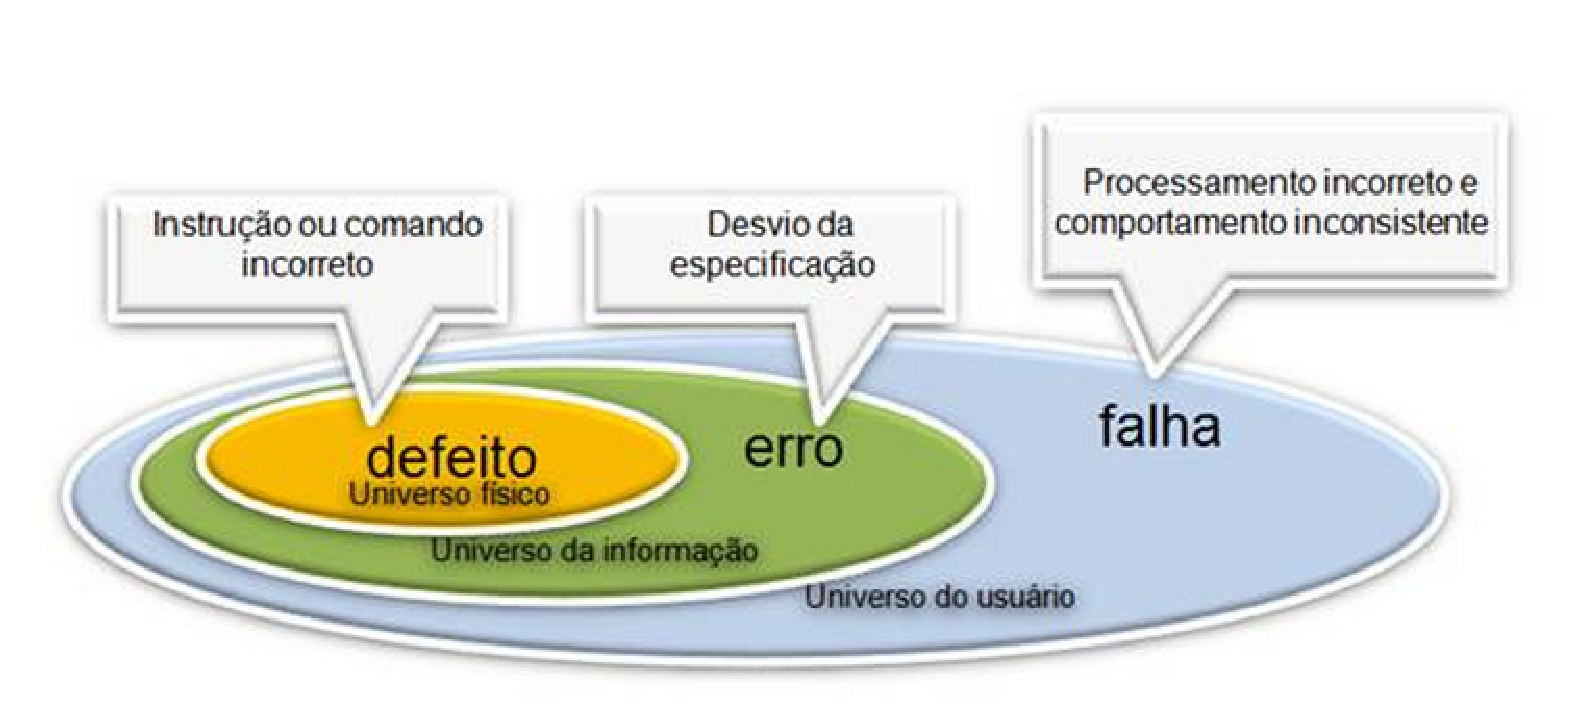
\includegraphics[width=0.9\textwidth]{figuras/defeitoErroFalha}
\caption{Defeito x Erro x Falha.}{Fonte:  \citeonline{neto2005}.}
\label{defeitoErroFalha}
\end{figure}

Teste e depuração são frequentemente confundidos, alguns acreditam até que são sinônimos, como foi mostrado anteriormente. A finalidade dos testes é mostrar que o programa tem erros, já o objetivo da depuração é encontrar o erro ou equívoco que levou ao fracasso do programa. Teste começa com condições conhecidas, utiliza procedimentos pré-definidos, e tem resultados previsíveis. A depuração começa a partir de condições iniciais, possivelmente desconhecidas \cite{beizer1990}.

Os testes podem ser projetados a partir de um ponto de vista funcional ou de um ponto de vista estrutural. Os testes funcionais são sujeitos a entradas, e suas saídas são verificadas afim de encontrar, ou não, conformidades com o comportamento especificado. O usuário do software deve se preocupar apenas com as funcionalidade e características \cite{beizer1990}.

Caixa-preta ou teste funcional:  “Teste de que ignora o mecanismo interno de um sistema ou componente e se concentra exclusivamente nas saídas geradas em resposta a entradas selecionadas e condições de execução” \cite{ieee}.

No método caixa-preta,como o próprio nome revela, vemos o programa como uma caixa preta. Seu objetivo é ser completamente indiferente sobre o comportamento interno e estrutura do programa. Em vez disso, se concentra em encontrar circunstâncias em que o programa não se comportam de acordo com as suas especificações\cite[pág.~13]{myers2004}.

Caixa-branca ou teste estrutural: “Testes que leva em conta o mecanismo interno de um sistema ou componente” \cite{ieee}.

 As conotações indicam adequadamente que você tem total visibilidade do funcionamento interno do produto de software, especificamente, a lógica ea estrutura do código \cite[pág.~1]{williams2006}.

Os testes são realizados em diferentes níveis, envolvendo o todo o sistema ou parte dele. São quatro níveis de teste: os teste de unidade, de integração, de sistema e de aceitação, como mostrado na figura \ref{nivelTeste} \cite[pág.~18]{naik2008}.

\begin{figure}[htp]
\centering
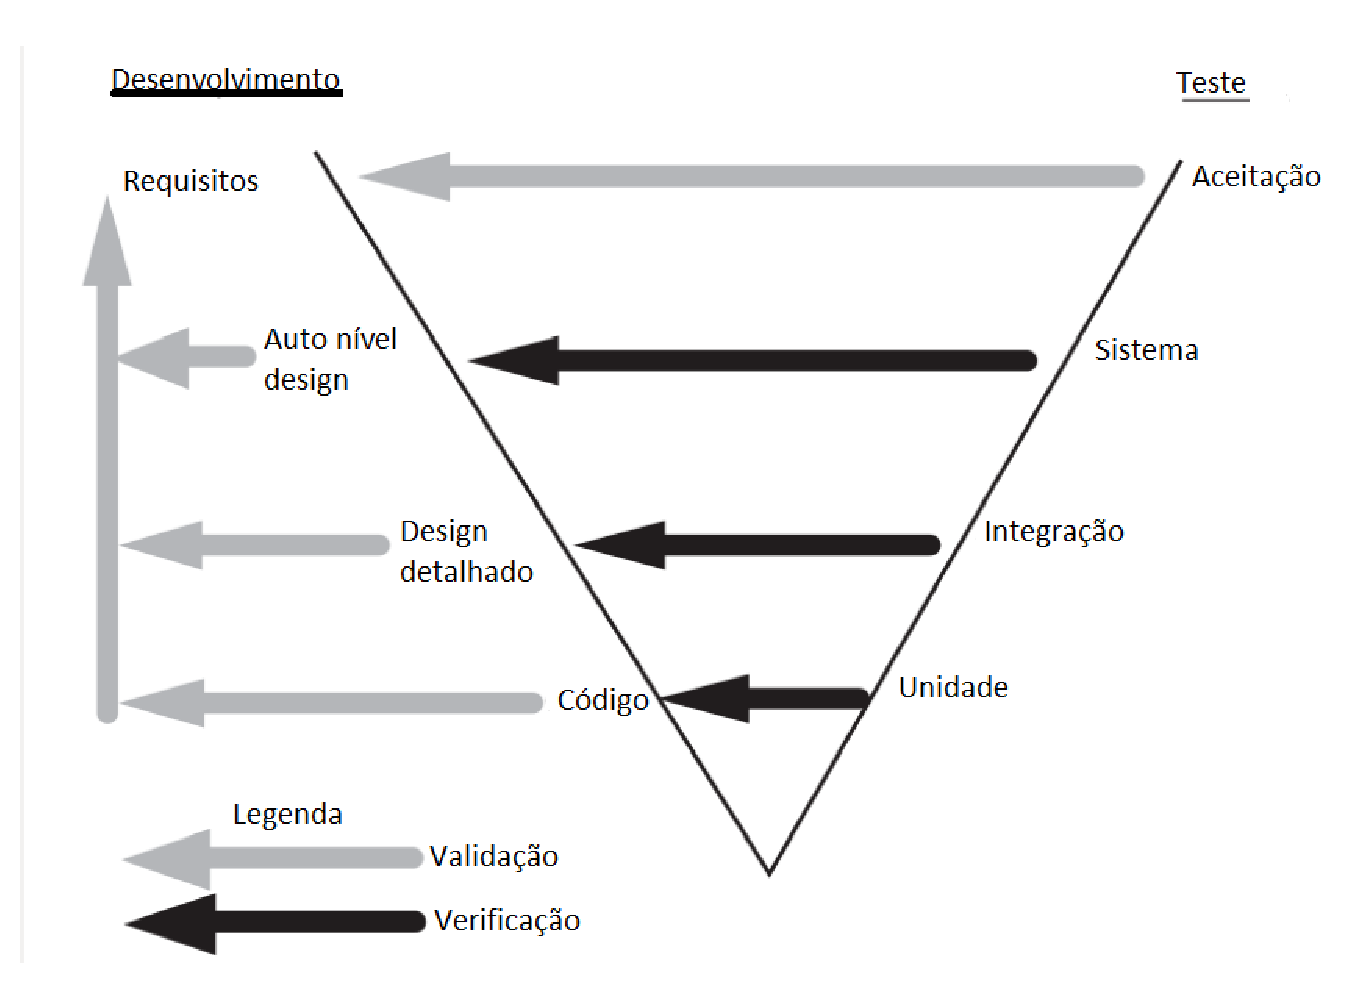
\includegraphics[width=0.9\textwidth]{figuras/nivelTeste}
\caption{Níveis de teste e seu desenvolvimento.}{Fonte: \citeonline[pág.~18]{naik2008}.} 
\label{nivelTeste}
\end{figure}

\subsection{Testes Unitários}

"Os testes de hardware individuais ou unidades de software ou grupos de unidades relacionadas" \cite{ieee}.

Testa-se unidades individuais do programa, como as funções, métodos ou classes, de forma isolada. Depois de garantir que as unidades funcionam de forma satisfatória, os módulos são montados para a construção de sub-sistemas maiores, seguindo técnicas de teste de integração \cite[pág.~18]{naik2008}.

Estes testes devem ser capazes de examinar o comportamento do código sob as mais variadas condições, ou seja, como o código deve se comportar se determinado parâmetro for passado (ou não), o que ele retorna se determinada condição for verdadeira, os efeitos colaterais que ele causa durante a sua execução, se determinada exceção é lançada \cite{thiago2001}.

O teste de unidade é importante para garantir que o código é sólido antes de ser integrado com outro código. Uma vez que o código está integrado na base de outro código, a causa de uma falha é mais difícil de ser encontrado \cite{williams2006}.

\subsection{Teste de integração}

“Testes em que componentes de software, componentes de hardware, ou ambos são combinados e testados para avaliar a interação entre eles” \cite{ieee}.

Seu objetivo é a construção de um sistema razoavelmente estável que pode suportar o rigor dos testes de nível de sistema \cite[pág.~18]{naik2008}.

O teste  efetuado de modo incremental através da combinação de módulos em etapas. Em cada etapa um módulo é adicionado à estrutura do programa, assim o teste se concentra neste módulo recém-adicionado. Depois de ter sido demonstrado que um módulo integra adequadamente com a estrutura do programa, um outro módulo é adicionado, e o teste continua. Este processo é repetido até que todos os módulos foram integrados e testados \cite[pág.~134]{lewis2009}.

Os casos de teste são escritos para examinar explicitamente as interfaces entre as diversas unidades. Estes casos de teste podem ser de caixa preta, em que o testador entende que um caso de teste requer várias unidades do programa para interagir. Como alternativa, têm-se os casos de teste caixa-branca que são escritos para exercer explicitamente as interfaces que são conhecidos para o testador \cite{williams2006}.

\subsection{Teste de Sistema}

“Testes conduzidos em um sistema completo e integrado para avaliar a conformidade do sistema com os requisitos especificados” (IEEE 610, 1990).

Teste de sistema verifica se as funções foram realizados corretamente. Também verifica se certas características não funcionais estão presentes. Alguns exemplos incluem de características não funcionais: testes de usabilidade, testes de desempenho, testes de stress, testes de compatibilidade \cite[pág.~134]{lewis2009}.

Uma pessoa que realiza teste de sistema deve ser capaz de pensar como um usuário final, o que implica uma profunda compreensão das atitudes e do ambiente do usuário final e de como o programa será usado. Então, se possível, um bom candidato a testador é um ou mais usuários finais. No entanto, o usuário final típico não têm a habilidade ou conhecimento para realizar muitas das categorias de testes, logo uma equipe de teste de sistema ideal pode ser composto por alguns especialistas de teste de sistema profissionais (pessoas que  passam a vida realizando testes do sistema), um  ou dois usuários representantes finais, um engenheiro de fatores humanos, e os principais analistas originais ou designers do programa \cite[pág.~104]{myers2004}.

\subsection{Teste de Aceitação}

“Teste formal realizado para permitir que um usuário, cliente ou outra entidade autorizada, para determinar se a aceita um sistema ou componente” \cite{ieee}.

Antes de instalar e utilizar o software na vida real outro último nível de teste deve ser executado: o teste de aceitação. Aqui, o foco está no cliente de e na ótica do usuário. O teste de aceitação pode ser a única prova de que os clientes estão efetivamente envolvidos \cite[pág.~61]{spillner2014}.

Geralmente, é realizada por um cliente ou usuário final do programa e, normalmente, não é considerada a responsabilidade da organização de desenvolvimento. No caso de um programa contratado, a organização contratante (usuário) realiza o teste de aceitação, comparando a operação do programa com o contrato original. Como é o caso de outros tipos de testes, a melhor maneira de fazer isso é criar casos de teste que tentam mostrar que o programa não atende o contrato, se esses casos de teste não forem bem sucedidos, o programa é aceito \cite[pág.~104]{myers2004}.  

\section{Qualidade de Software}

\begin{citacao}
“Qualidade é um termo que pode ter diferentes interpretações e para se estudar a qualidade de software de maneira efetiva é necessário, inicialmente, obter um consenso em relação à definição de qualidade de software que está sendo abordada” \cite[pág.~11]{braga2012}.
\end{citacao}

A qualidade de software é classificada em fatores internos e externos. Fatores externos são aqueles em que usuários comuns conseguem detectar, como por exemplo, a velocidade do software ou a facilidade de uso. Os fatores externos agregam bastante valor ao usuário final, mas um bom caminho para assegurar que os fatores externos terão qualidade é caprichar na construção dos fatores internos. Portanto, técnicas de qualidade interna, como análise de qualidade de código fonte, são meios para atingir a qualidade externa \cite[pág.~4]{bueno2011}.

\subsection{Métricas de Qualidade de Código Fonte}

Conceitos de qualidade são imprecisos e difíceis de serem aceitos em diversos contextos. No contexto de desenvolvimento de software, métricas de qualidade de código possuem o intuito de mensurar qualidade do produto de software \cite[pág.~1]{bueno2011}.

As métricas de qualidade de código fonte podem ser objetivas ou subjetivas. As métricas subjetivas são obtidas através de regras bem definidas. As métricas subjetivas depende do sujeito que está realizando a medição. As métricas objetivas podem ser calculadas a partir de uma análise estática de código fonte de um software. Os resultados das métricas podem ser mapeados em intervalos com o intuito de serem interpretados quando analisados \cite[pág.~14]{meirelles2013}

As métricas de qualidade de código fonte possuem papel fundamental no monitoramento e controle nas atividades de codificação e testes, realizados quase sempre por equipes que possuem diferentes formas de pensar e de realizar o trabalho criativo de codificação \cite[pág.~341]{sommerville}.

\begin{citacao}
“Ao contrário de outras engenharias, a engenharia de software não é baseada em leis quantitativas básicas, medidas absolutas não são comuns no mundo do software. Ao invés disso, tenta-se derivar um conjunto de medidas indiretas que levam a métricas que fornecem uma indicação de qualidade de alguma representação do software. Embora as métricas para software não sejam absolutas, elas fornecem uma maneira de avaliar qualidade através de um conjunto de regras definidas” \cite[pág.~]{bueno2011}.
\end{citacao}

\subsection{Análise Estática de Código Fonte}

A análise estática de código é um processo automatizado realizado por uma ferramenta sem a necessidade de execução do programa ou software a ser verificado \cite[pág.~64]{chess2007}.

Na utilização da análise estática de código fonte, falhas são descobertas mais cedo no desenvolvimento, antes do programa ser executado, ainda em versões de testes. A real causa dos defeitos é revelada e não apenas suas consequências \cite[pág.~19]{melo2011}.

\citeonline{filho}, define um intervalo de interpretação das métricas de qualidade de código fonte para se saber se a qualidade do código está preocupante, regular, boa ou excelente conforme a figura \ref{intervalosMetricas}.

\begin{figure}[htp]
\centering
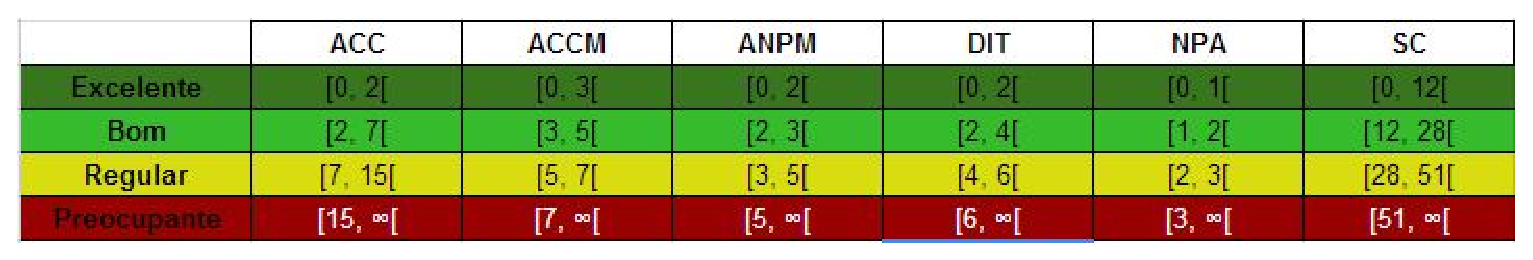
\includegraphics[width=0.9\textwidth]{figuras/intervalosMetricas}
\caption{Intervalo para interpretação das métricas.}{Fonte: \citeonline{filho}.} 
\label{intervalosMetricas}
\end{figure}

\subsection{Ferramentas de Análise Estática}

Ferramentas de análise estática de código fonte varrem o código fonte e detectam possíveis anomalias. Também pode ser usados como parte de um processo de inspeção \cite[pág.~345]{sommerville}.

Obter os dados e extrai-los para análise estática de código fonte, não é uma tarefa trivial e requer a utilização de ferramentas automatizadas \cite[pág.~2]{meirelles2013}

As métricas de qualidade de código fonte podem ser obtidas através do uso de uma ou mais ferramentas de extração de métricas. Existem diversas ferramentas para realização dessa atividade, mas não é possível afirmar que uma ferramenta é melhor que outras. Todas possuem pontos fortes e fracos. Para se escolher uma ferramenta de análise estática, deve-se analisar o contexto em que as mesmas estão inseridas como, por exemplo, a linguagem do projeto a ser analisado \cite{millani2013}.